\chapter{Grundlagen}

Dieses Kapitel beinhaltet technologische sowie konzeptionelle Grundlagen für das \\
Verständnis der untersuchten Softare Anwendungen sowie für die Testing Methode der final ausgewählten Anwendung.

\section{Groupwaresysteme}

Groupwaresysteme sind Softwareandwendungen, die die Zusammenarbeit von Benutzern mit verschiedenen Tools zur gemeinsamen Kommunikation und Organisation unterstützen.
Dabei werden gewöhnlich Funktionalitäten wie Kalender, Terminplanung, E-Mail und Kontaktmanagement geliefert.
\\
Die grundsätzliche Funktionsweise einiger essenzieller Funktionen von Groupwar-Systemen wird im Folgenden anhand von Screenshots aus Microsoft Outlook Live beispielsweise dargestellt und erklärt:
\begin{figure}[H]
    \centering
    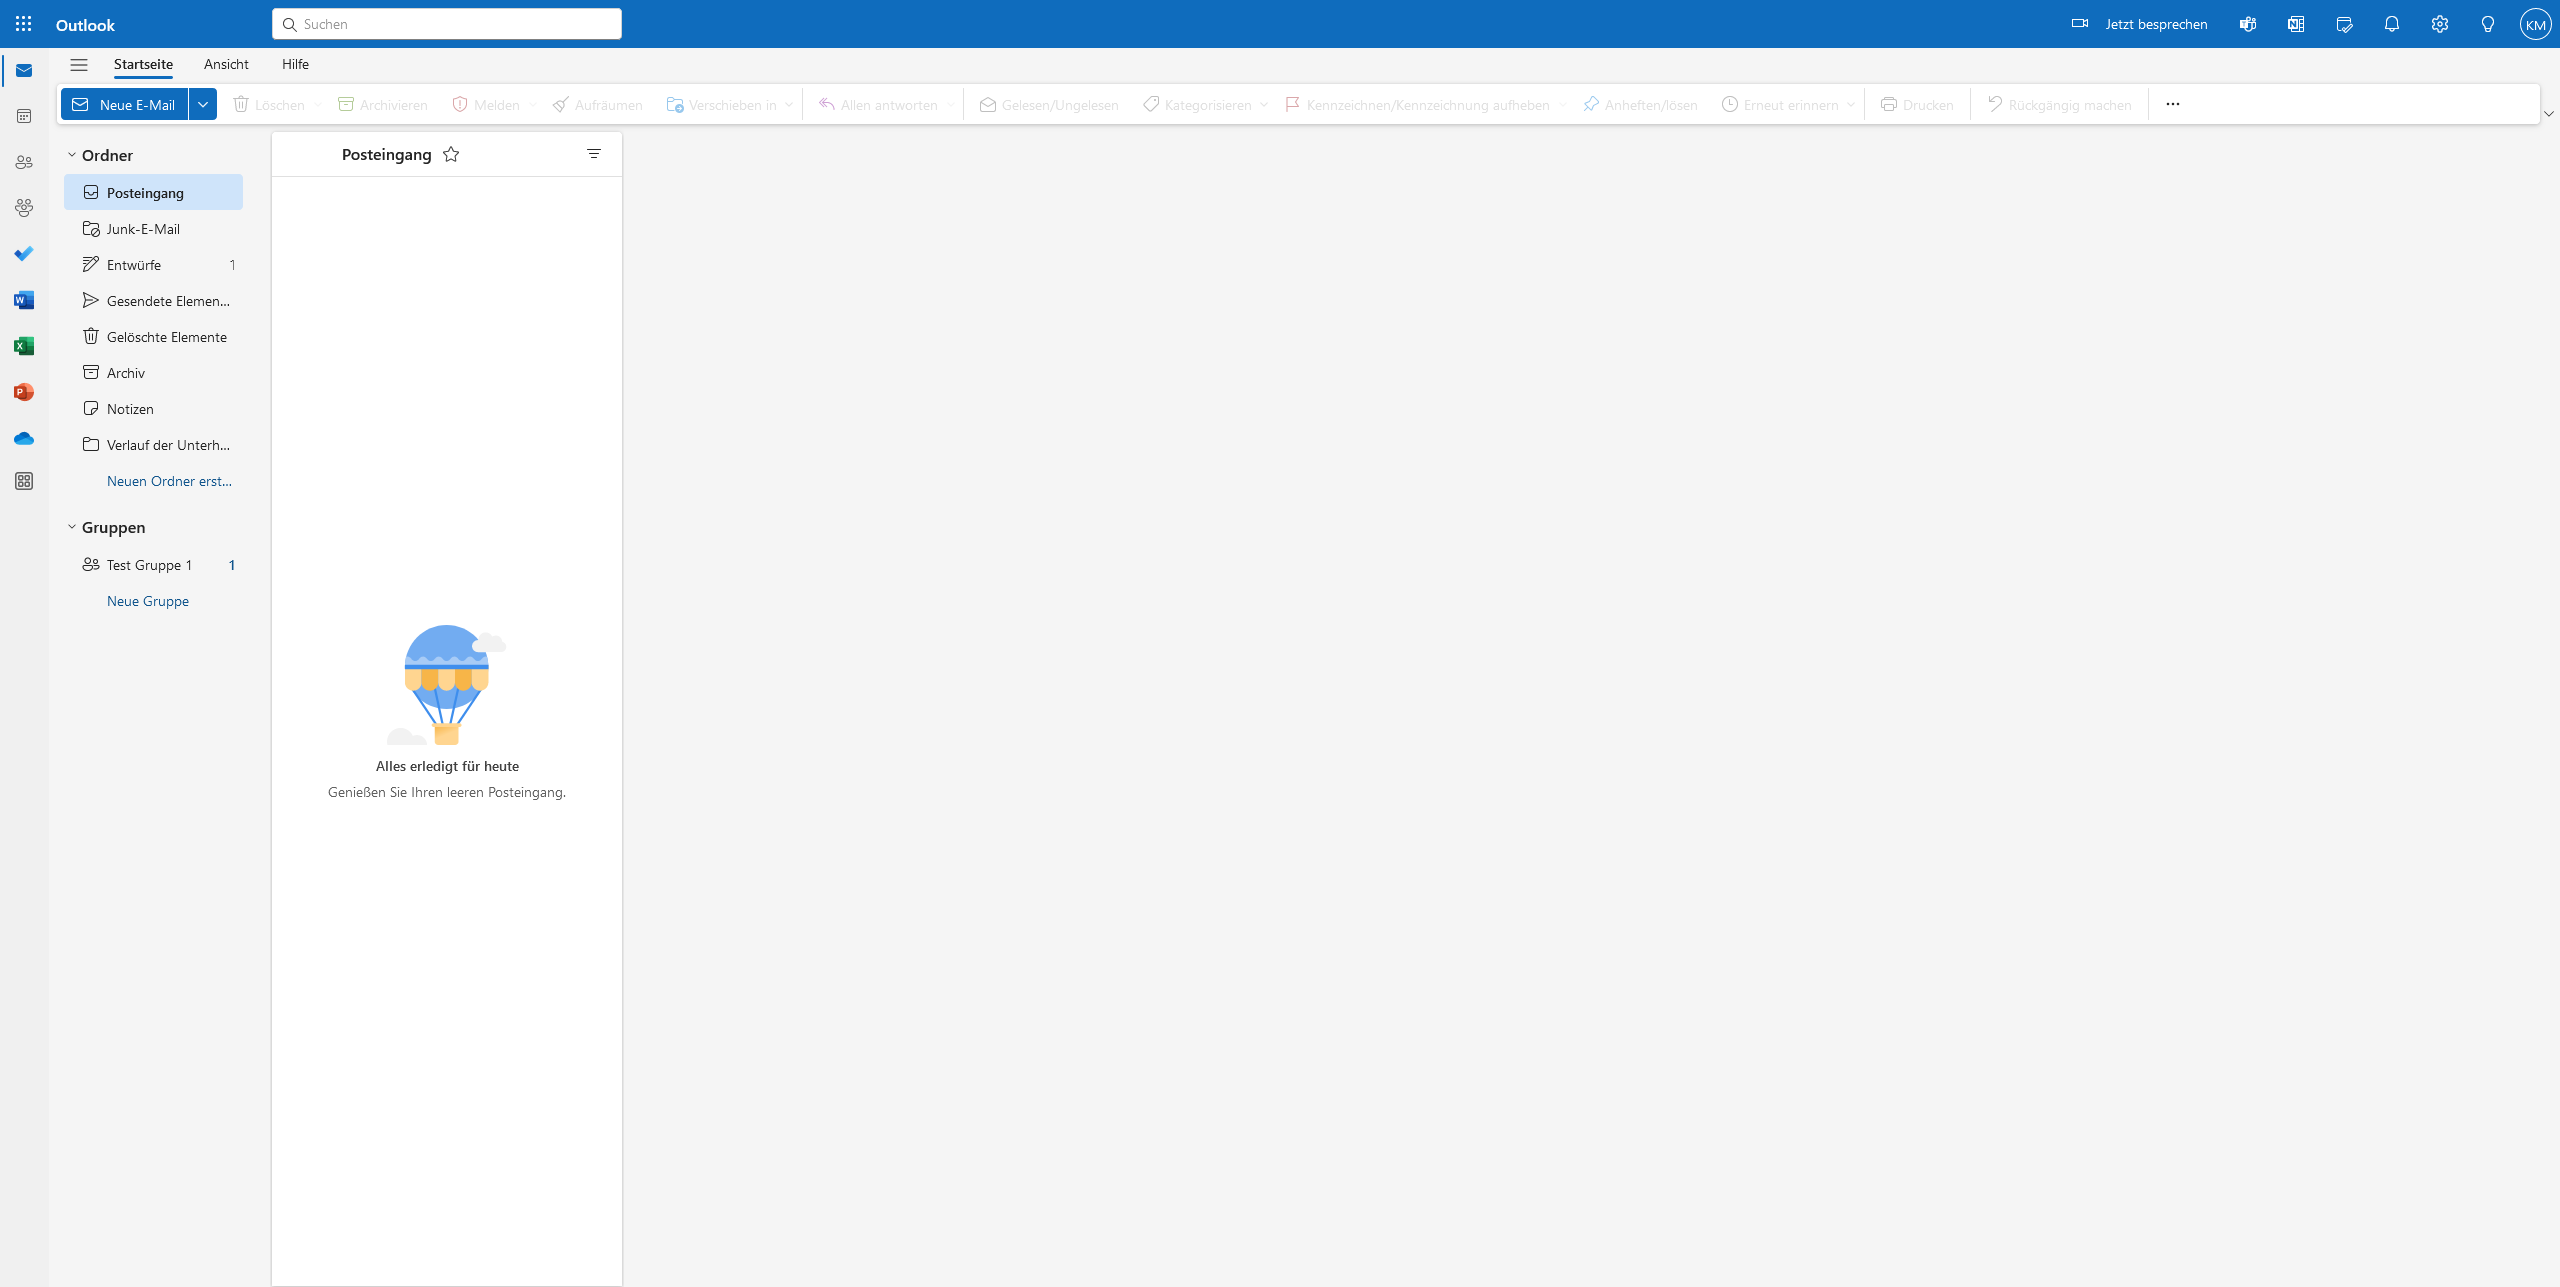
\includegraphics[width=0.75\textwidth]{images/OutlookLive_Mail1.png}
    \caption{OutlookLive Mail}
    \label{fig:outlook-live-mail}
\end{figure}
Die erste Hauptfunktion die Groupwaresysteme erfüllen ist, wie in Abbildung \ref{fig:outlook-live-mail} beispielhaft anhand Outlook Live dargestellt, das anbieten eines E-Mail Clients über den E-Mails empfangen, versendet und verwaltet werden können.
Dabei sollten sich auch mehrere E-Mail Postfächer gleichzeitig hinzugefügt werden können.


\begin{figure}[H]
    \centering
    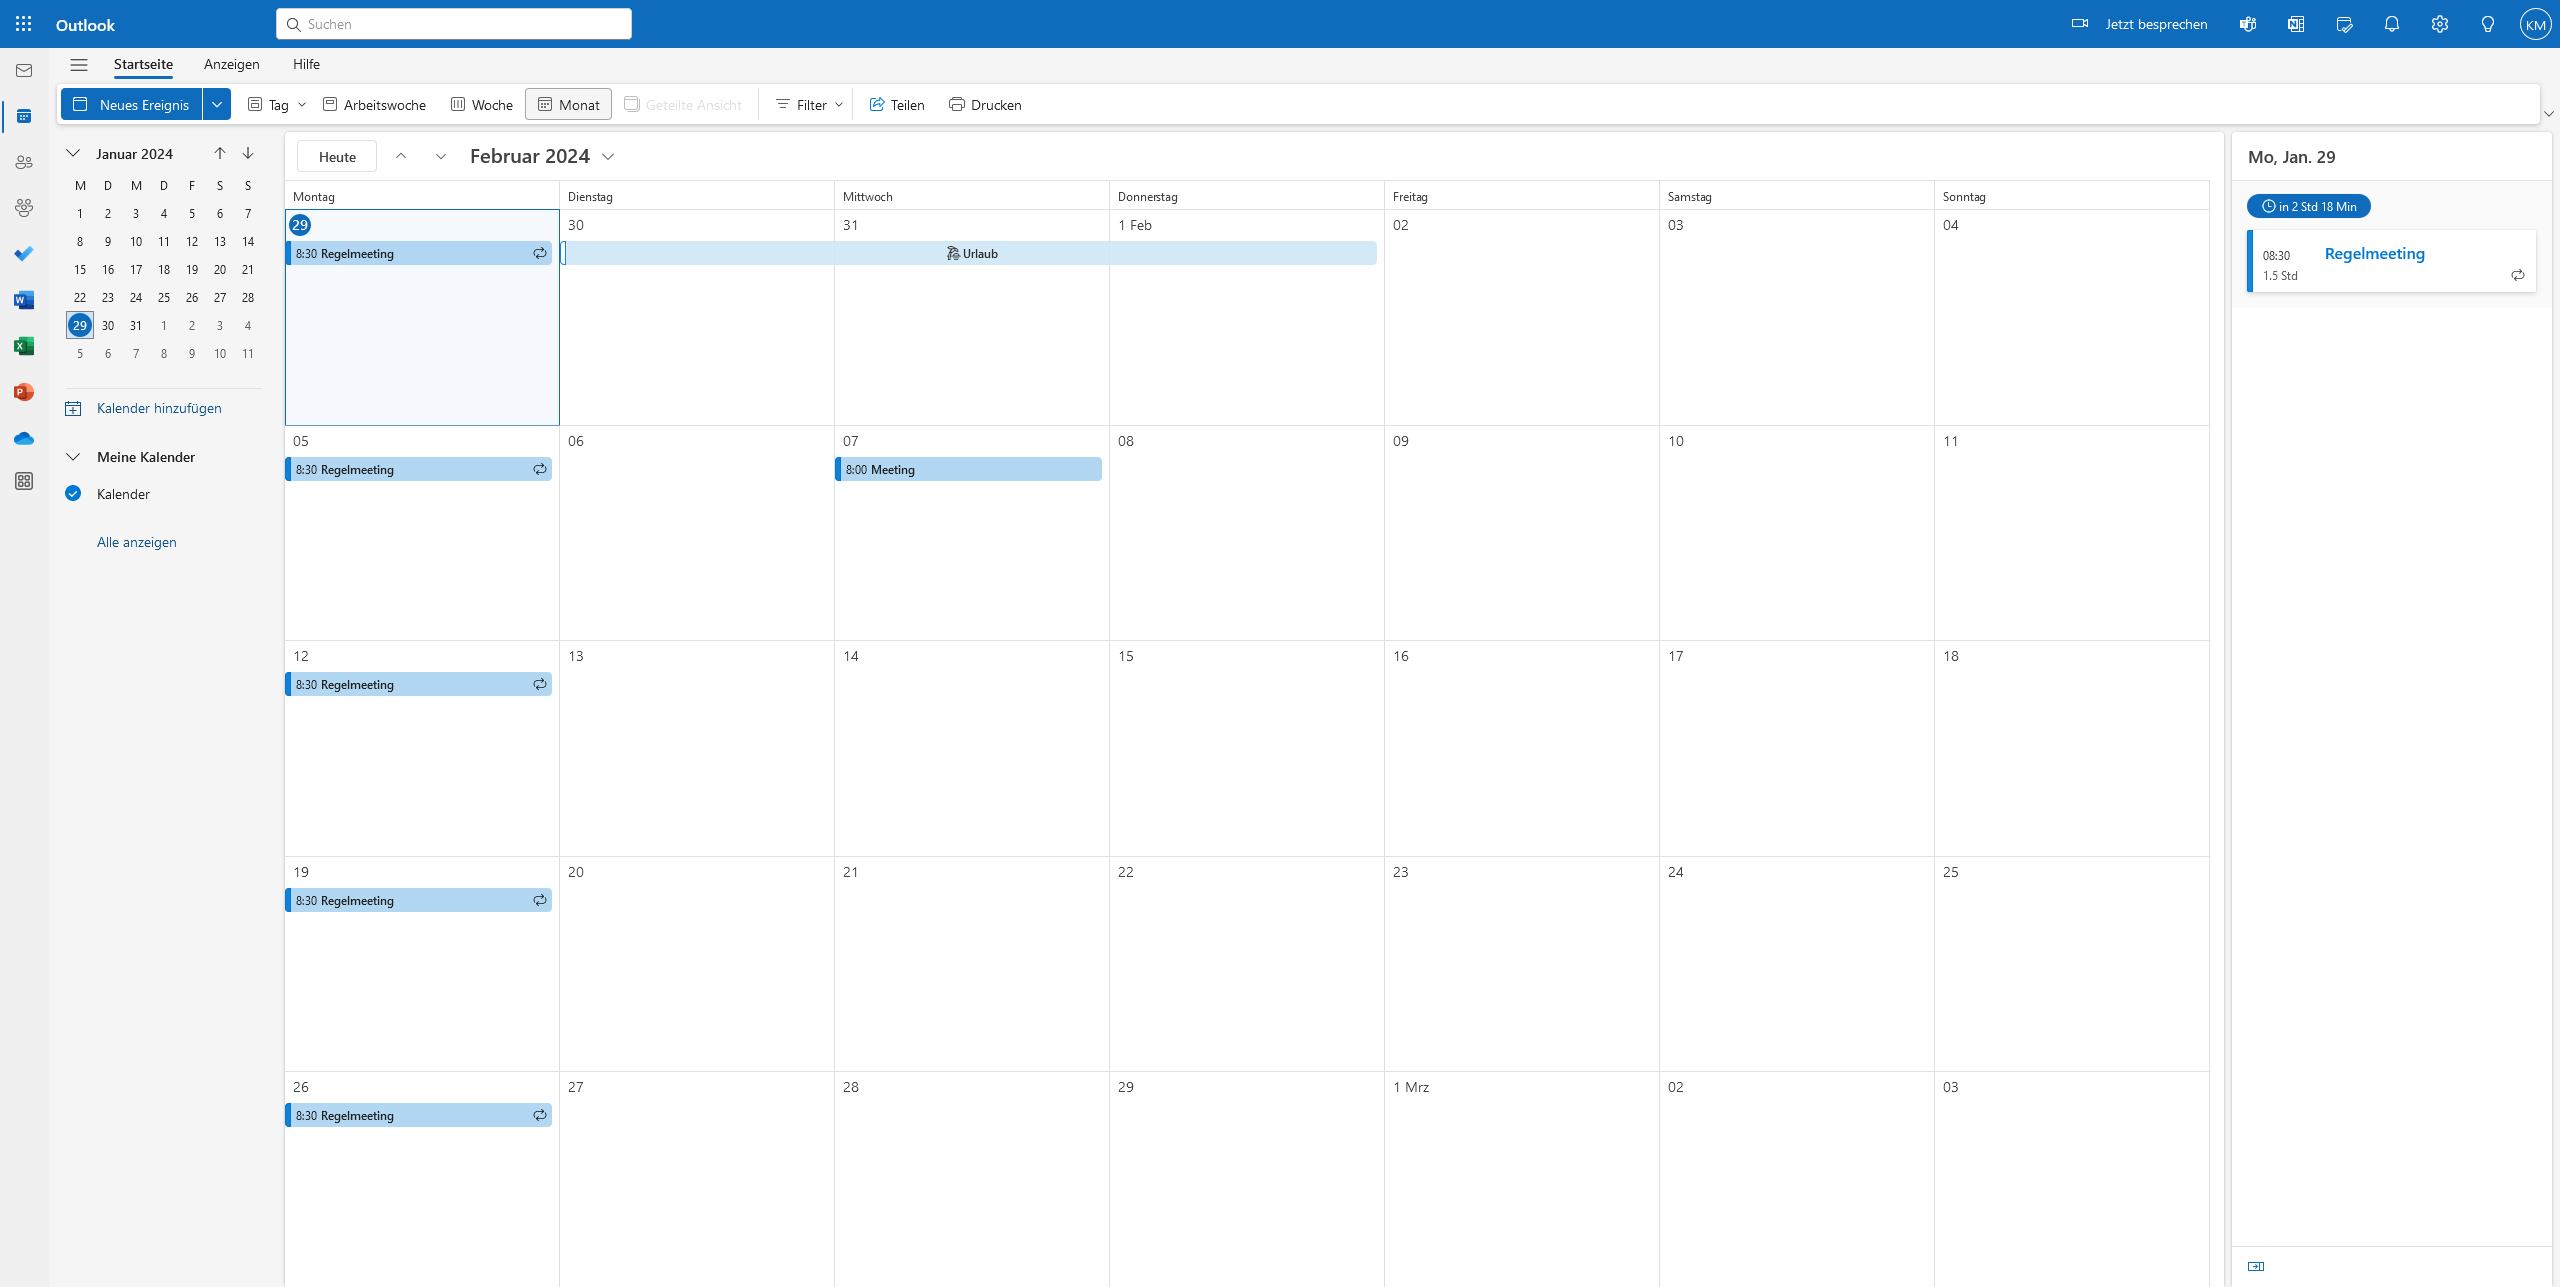
\includegraphics[width=0.75\textwidth]{images/OutlookLive_Calender1.png}
    \caption{OutlookLive Calender}
    \label{fig:outlook-live-calender}
\end{figure}

Eine weitere Hauptfunktion von Groupwaresystemen ist ein Kalender, der Nutzern wie in Abbildung \ref{fig:outlook-live-calender} Terminplanung in Form eines Kalenders mit Ereignisplanung ermöglicht.
Die Terminplanung sollte das Einladen von anderen Nutzern ermöglichen um die Zusammenarbeit und Organisation der Nutzer miteinander zu vereinfachen.
Dabei sollten auch Regeltermine, also Termine die sich regelmäßig wiederholen erstellt werden können.

\begin{figure}[H]
    \centering
    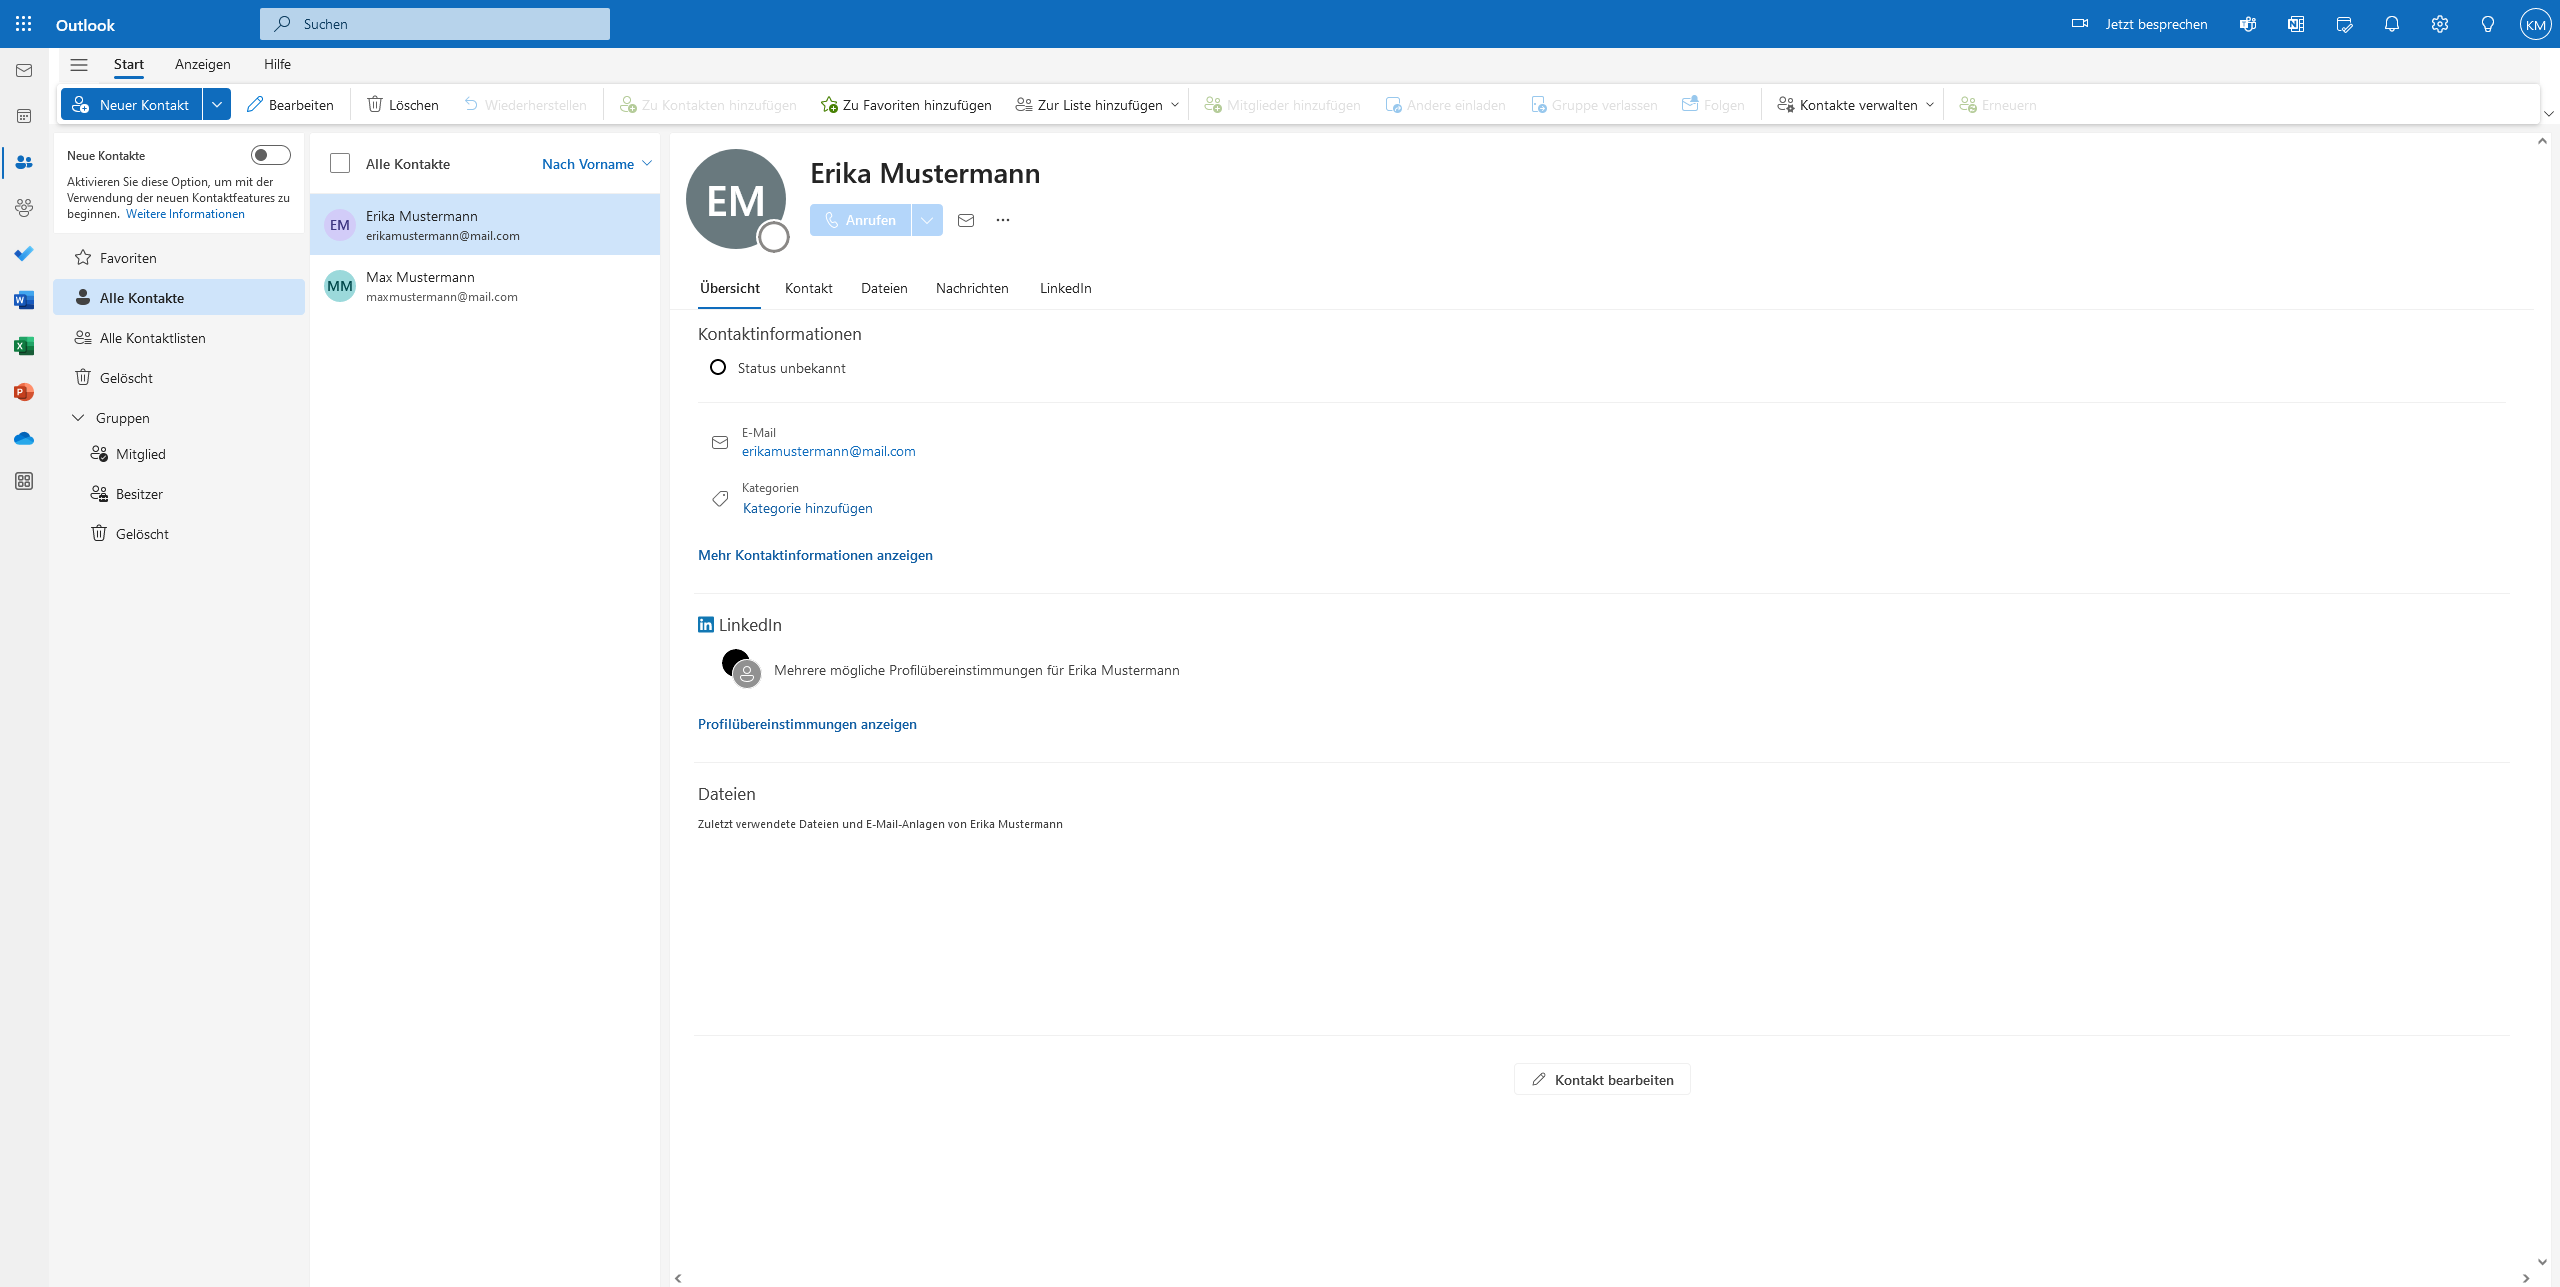
\includegraphics[width=0.75\textwidth]{images/OutlookLive_Contacts.png}
    \caption{OutlookLive Contacts}
    \label{fig:outlook-live-contacts}
\end{figure}

Kontakte sind eine esentieller Bestandteil von Groupwaresystemen um die Vernetzung innerhalb von Arbeitsgruppen zu organisieren.
Durch sie sollte die Kontaktaufnahme zu anderen Gruppenmitgliedern so einfach wie möglich gestaltet werden.
Im Beispiel von OutlookLive kann man wie in Abbildung \ref{fig:outlook-live-contacts} gezeigt direkt vom Kontakt einer Person diese Person über Nachrichten, Anrufe oder E-Mail kontaktieren.


\section{Playwright}

Die Open-Source-Bibliothek Playwright wurde Anfang 2020 von Microsoft veröffentlicht und ermöglicht es, Browser automatisiert zu steuern und dadurch automatisierte Tests für Webanwendungen durchzuführen oder Websites zu scrapen.
Dabei bietet Playwright ein Application-Programming-Interface (API) für die Programmiersprachen JavaScript, TypeScript, Python, .NET und Java, sowie eine Vielzahl von Funktionen, die das Testen von Webanwendungen erleichtern.
Beispielsweise kann mit Playwright Codegen die eigene Interaktion mit einer Webanwendung augezeichnet und als Code exportiert werden, der dann als Test für die ausgeführte Interaktion verwendet werden kann.
So können effizient Frontend-Tests für eine Vielzahl von Anwendungen implementiert werden.
\autocite[Quelle:][]{playwright}
\\
\\
Im Fall der Studienarbeit wurde Playwright verwendet, um automatisierte End-to-End Tests für das final ausgewählte Groupware-System durchzuführen.
Dabei werden Frontend-Tests implementiert, die typische Interaktionen mit der Benutzeroberfläche simulieren.
So können beispielsweise Formulare ausgefüllt oder Buttons angeklickt werden, womit ein Nutzer-Login und das anschließende Aufrufen der Mails des Nutzers simuliert werden kann.
\\
Deckt man mit diesen Tests alle Funktionsbereiche des Groupwaresystems ab, kann man durch das Ausführen der Tests sicherstellen, dass die Anwendung nach einer Änderung noch wie erwartet funktioniert.
Auch falls die Anwendung in Zukunft unerwartete Ausfälle generiert, können diese durch flächendeckende Tests genauer erkannnt werden, da sofort ersichtlich ist, welche Bereiche des Systems noch funktionieren und welche nicht.
Geht beispielsweise der zuvor erwähnte Test des aufrufen der Mails schief, gibt es mit hoher Wahrscheinlichkeit ein Problem mit der Verbindung zum Mail Server.
\\
Zudem können solche Tests in Playwright in verschiedenen Browsern (Chromium, Firefox, Safari) ausgeführt werden, wodurch die Funktionalität der Anwendung auch auf verschiedenen Browsern sichergestellt und kontinuierlich getestet werden kann.
Da die Groupware von einer Vielzahl von Systemen zugänglich sein soll, ist diese Funktion ein essentieller Bestandteil der Testanforderungen.








